\section{Introducción}

\subsection{Motivación}

La emisión de radiación electromagnética ha permitido descubrir la composición, cinemática y distribución del medio intergaláctico y estrellas.

La nubes frías de hidrógeno gaseoso no emiten luz visible sino ondas de radio. Estas nubes son importantes porque pueden indicar el lugar de nacimiento de estrellas.

La radioastronomía usa radiotelescopios que captan ondas de radio, de longitudes de aproximadamente \SI{1}{\centi\meter} a \SI{10}{\meter}. Favorablemente, estas ondas coinciden con una ventana en la atmósfera, permitiendo su detección. A pesar de esto, la atmósfera sigue teniendo opacidad, dando lugar a errores en la medición de las señales, al igual que el error sistemático provocado por el instrumento mismo y su receptor en la antena.

Este informe trata sobre, primero, ciertas calibraciones para el radiotelescopio que permiten mejorar la precisión de las mediciones y, en segundo lugar, sobre el estudio de la nebulosa de Orión.

\subsection{Estructura del Informe}

Las siguientes subsecciones introducen el radiotelescopio y el instrumento utilizado en este informe, junto con una descripción de un espectro de potencia medida y importancia de las calibraciones.

Las secciones \ref{sec:hotcoldtest} y \ref{sec:antennadipping} tratan sobre dos calibraciones para el telescopio, el Hot--Cold Test y Antenna Dipping, respectivamente, incluyendo un marco teórico, presentación de los datos medidos y cálculo de calibraciones, junto con la comparación con respecto a las provistas por el software del radiotelescopio.

La sección \ref{sec:observaciones} introduce el objeto celeste observado, junto con los espectros, temperatura de la fuente y errores asociados.

Finalmente, la sección \ref{sec:conclusiones} presenta las conclusiones del informe, estableciendo que las calibraciones son importantes para mejorar la precisión de instrumento y que los datos del experimento pudieron ser afectador por factores climáticos pues presentar error.

Además, la sección \ref{sec:anexo} es un anexo con los códigos utilizados para los cálculos y gráficos, que también están disponibles en \url{https://github.com/camilo-nb/AS3201-tareas/tree/main/tarea1}.

\subsection{El radiotelescopio}\label{sec:radiotelescopio}

Un radiotelescopio es una antena especializada en captar ondas de radio. Generalmente tiene una antena parabólica, con un reflector principal que redirige la radiación recibida del cielo, concentrándola en un reflector secundario pequeño y contrapuesto, que a su vez redirige la señal concentrándola en un pequeño receptor en la bocina de la antena.

La potencia espectral $w$ recibida por unidad de ancho de banda es,
\begin{equation}
w=\frac{1}{2}A_\textnormal{e}\iint_\Omega{B(\theta,\phi)P_n(\theta,\phi)\dd{\Omega}}\label{eq:w}
	,\end{equation}
donde $A_\textnormal{e}$ es la apertura efectiva de la antena, $B$ es el brillo del cielo, $P_n$ es el patrón de potencia normalizado de la antena que mide de la respuesta de sus lóbulos como función de los ángulos, y $\dd{\Omega}$ es el elemento infinitesimal de ángulo sólido del cielo. Además, el factor $1/2$ es debido a que la antena es responsable de una sola componente de polarización de la radiación.

\subsection{Radiotelescopio MINI}\label{sec:mini}

Los experimentos de este informe se realizan gracias a las mediciones hechas por el equipo docente mediante el radiotelescopio Southern Millimeter-Wave Telescope (ver figura \ref{fig:mini}), que ha permitido importantes investigaciones como un mapeo extenso y uniforme del carbolo interestelar de toda nuestra galaxias. Actualmente se usa para observaciones docentes, como la de este curso e informe.

Este telescopio se denomina MINI por su pequeño tamaño. Está en su propio domo en el Observatorio Astronómico Nacional, en la cima del cerro Calán. Su antena tiene un diámetro de \SI{1.2}{\meter}. Tiene instalado un amplificador HEMT (High Electro Mobility Transistor) en la primera etapa de recepción que proporciona una mejor relación señal a ruido. Tiene dos espectrómetros de banco de filtros con 256 canales cada uno, que captan ondas electromagnéticas con frecuencias d \SI{86}{\giga\hertz} a \SI{115}{\giga\hertz}, con resoluciones respectivas de \SI{0.1}{\mega\hertz} y \SI{1}{\mega\hertz}.

\subsection{Espectros de absorción}

La potencia recibida (ecuación \ref{eq:w}) se puede recolectar a través de todos los canales del radiotelescopio, cada uno con una resolución determinada y un ancho de banda respectivo, permitiéndo graficarla en lo que se denomina espectro de absorción, como el que muestra la figura \ref{fig:spectrum}, que es para la luz visible pero sigue siendo ilustrativo para cualquiera. Las frecuencias o longitudes de ondas, adicionando su corrimiento debido al efecto Doppler, se pueden interpretar como velocidades radiales.

Una línea de absorción corresponde a un mínimo local preponderante en la curva del espectro y se producen porque los átomos en la línea de visión de la fuente se interponen en los fotones y absorben la energía para excitar sus electrones. Un ejemplo de absorción ocurre en las nubes de hidrógeno, que tienen temperaturas frías, y suelen indicar formación de estrellas. Se denomina continuo al espectro sin líneas de absorción.

Una línea de emisión corresponde a un máximo local preponderante en la curva del espectro y se produce por los fotones emitidos por las fuentes y los átomos que las componente. Un ejemplo de emisión ocurre en los cuásares y el hidrógeno que producen, estando a una muy alta temperatura.

\begin{figure}[p]
	\centering
	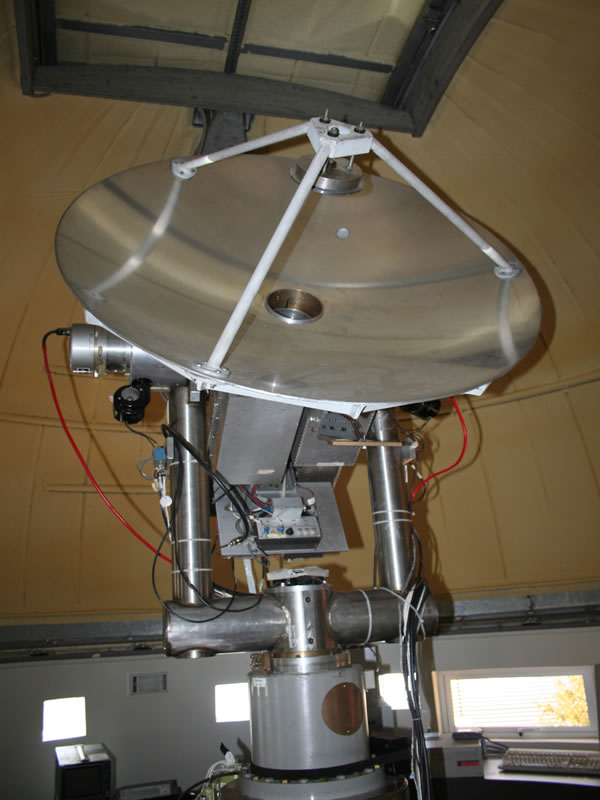
\includegraphics[width=3.25in]{rsc/mini.jpg}
	\caption{Radiotelescopio MINI (Imagen: DAS, FCFM)}
	\label{fig:mini}
\end{figure}

\begin{figure}[p]
	\centering
	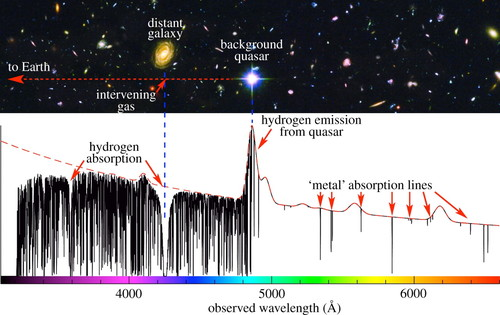
\includegraphics[width=3.25in]{rsc/spectrum.jpg}
	\caption{Espectro de absorción de un cuásar distante (Imagen: Joe Liske, ESO)}
	\label{fig:spectrum}
\end{figure}